\documentclass[12pt,a4paper]{report}

% - BASIC PACKAGES -
\usepackage[utf8]{inputenc}
\usepackage[english]{babel}
\usepackage{amsmath, amssymb}
\usepackage{graphicx}
\usepackage{geometry}
\usepackage{titlesec}
\usepackage{enumitem}
\usepackage{caption}
\usepackage{indentfirst}
\usepackage{microtype}
\usepackage{tikz}
\usepackage{tabularx}
\usepackage{float}

\usetikzlibrary{shapes.geometric, arrows.meta, positioning, shadows}

\setlength{\parindent}{1cm}

% Values still to be filled in by the authors (shown in red in the PDF)
\newcommand{\tofill}[1]{\textcolor{red}{[#1]}}

% - LINKS AND INTERACTIVE TABLE OF CONTENTS -
\usepackage{hyperref}
\hypersetup{
    colorlinks=true,
    linkcolor=black,
    pdftitle={OctoBouncer Documentation},
    citecolor=blue,
}

\geometry{margin=2.5cm}

% Chapter style
\titleformat{\chapter}[display]
  {\normalfont\huge\bfseries}{\chaptertitlename\ \thechapter}{20pt}{\Huge}
\titlespacing*{\chapter}{0pt}{0pt}{40pt}

\begin{document}

% - TITLE PAGE -
\begin{titlepage}
    \centering
    \vspace*{3cm}
    {\Huge \textbf{OctoBouncer} \par}
    \vspace{1.5cm}
    {\Large Dynamic Balancing and Trajectory Control System \par}
    \vspace{4cm}
    {\large \textbf{Authors:} \par}
    \vspace{0.8cm}
    {\Large \textbf{Oana Datcu}} \\
    {\small Faculty of Mechanics and Mechatronics \par}
    \vspace{1cm}
    {\Large \textbf{Ivan Alexandru}} \\
    {\small Faculty of Automatic Control and Computer Science \par}
    \vspace{2cm}
    {\large \textbf{Coordinators:} \par}
    \vspace{0.8cm}
    {\Large \textbf{Assoc. Prof. Dr. Eng. Daniel Rosner}} \\
    \vspace{0.2cm}
    {\Large \textbf{Eng. Teodor Dicu}} \\
    \vspace{0.2cm}
    {\Large \textbf{Teaching Assist. PhD Cand. Eng. Vlad Stănescu}} \\
    \vfill
    {\large Year 2026 \par}
\end{titlepage}

\newpage
\pagenumbering{gobble}
\tableofcontents
\newpage
\pagenumbering{arabic}

% - CHAPTER 1: INTRODUCTION -
\chapter{Introduction}
\label{chap:intro}

The problem of balancing a spherical body on a flat surface, known in the specialized literature as ``Ball and Plate'' \cite{ball_plate_model}, is one of the complex problems in the field of control systems engineering. Although at first glance it seems a simple problem, it introduces an unstable nonlinear dynamics, in which any positioning error is affected by external factors.

The \textbf{OctoBouncer} project, having as its source of inspiration the project of the same name \cite{source_project}, proposes a modern approach to this paradigm, extending the limits from simple stabilization to trajectory tracking, with the dynamic control of momentum (bouncing the ball) as the long-term goal. Our objective was not only to keep the ball at a fixed point, but to transform the platform into a system capable of complex interactions, such as complex trajectories.

This achievement required close collaboration between two fundamental disciplines:

\begin{itemize}[leftmargin=2cm]
    \item \textbf{Mechatronics:} Designing a platform driven by four arms, with three degrees of freedom (pitch, roll and height), characterized by low mass and high rigidity, capable of executing sudden vertical accelerations without compromising angular precision.
    \item \textbf{Automatic Control:} Developing a distributed control system, in which high-frequency image processing (Raspberry Pi 5 \cite{rpi5}) is closely tied to a real-time system (Teensy 4.1 \cite{teensy41}) in order to estimate the state of the ball and generate commands for the motors with minimal latency.
\end{itemize}

Through OctoBouncer, we demonstrate how feedback control algorithms and image processing can be integrated into a robust physical system, capable of holding the manipulated object at a fixed point and of moving it along predefined trajectories; managing its kinetic energy as well is the next step of the project.

\chapter{Mechanical Design and Hardware \newline Implementation}
\label{chap:hardware}

The mechanical design of the \textbf{OctoBouncer} system evolved through an iterative process, with structural rigidity, efficient thermal management and easy maintenance as fundamental objectives. The chosen architecture is based on a redundant parallel robotic platform, a technical solution that offers a superior dynamic response compared to standard three-support-point configurations \cite{parallel_robot}. By using four independent actuation arms, the system manages to correct positioning errors in real time, ensuring increased stability of the platform plane even during translation movements, derived from the Stewart architecture \cite{ik_stewart}.

\begin{figure}[H]
   \centering
   \includegraphics[width=0.7\textwidth]{sistem_complet.png}
   \caption{\textit{Isometric representation of the complete OctoBouncer system in the final design stage.}}
\end{figure}

\section{Anatomy of the Actuation Arm and Kinematic Optimization}
The actuation arm is the most stressed component of the system, being designed to balance low mass with high mechanical strength. Its prototyping was carried out by 3D printing from \textbf{PET-G} \cite{petg_material}, a material chosen for its superior impact resistance and its ability to maintain tight assembly tolerances. Each arm integrates a complex hybrid structure: one active joint connected directly to the motor and three free joints.

From a technical standpoint, the elimination of mechanical backlash was achieved by integrating \textbf{precision bearings} at each pivot point. This decision was critical in preventing parasitic vibrations that could have destabilized the control algorithm at high frequencies. An important innovation compared to previous versions was the introduction of an additional joint on a perpendicular plane, positioned at the point of contact with the platform. This modification solved the diagonal mobility limitations, allowing the platform to execute complex trajectories without geometric constraints.

\begin{figure}[H]
   \centering
   \includegraphics[width=0.6\textwidth]{brat_cad.png}
   \caption{\textit{Arm detail: optimization of the joints and the perpendicular pivot point for extended mobility.}}
\end{figure}

\section{Chassis Integration and Component \newline Management}
The chassis of the system does not serve only as a structural support, but also as a casing and protection for the electronic components. The upper platform is made of \textbf{8 mm plexiglass}. We opted for this thickness because it offers optimal inertia for stability, while also having elastic properties that favor the rebound function of the ball.

Beyond the mechanical aspects, a major challenge was \textbf{thermal management}. Stepper motors tend to generate high temperatures during prolonged operation, which could lead to structural deformation of the polymer parts. To counter this phenomenon, we used metal brackets that absorb and dissipate the motors' heat, protecting the integrity of the PET-G base. Furthermore, the chassis design was provided with ventilation slots and dedicated air tunnels for the DM556 drivers \cite{dm556}, ensuring efficient active cooling under heavy loads.

\begin{figure}[H]
   \centering
   \includegraphics[width=0.6\textwidth]{section_pwr.png}
   \caption{\textit{Internal section: airflow architecture and ergonomic layout of the power components.}}
\end{figure}

Accessibility of the system was another priority in the design stage. We designed a \textbf{slider-type system} and interior channels for the efficient arrangement of the cables, facilitating quick access to the connections without the need to disassemble the arms. This approach reduces maintenance time and eliminates the risk of power or data wires interfering with the moving elements of the robot.

\begin{figure}[H]
   \centering
   \includegraphics[width=0.55\textwidth]{mecanism_sliding.png}
   \caption{\textit{Detail of the sliding mechanism designed for quick access to the central computing unit and wiring.}}
\end{figure}

\section{Evolutionary Analysis of the Prototype}
The transition from the initial version to the current \textbf{OctoBouncer} model involved a series of fundamental modifications. The first version suffered from low stability due to a center of mass that was too high and a lack of space for managing the wiring. The table below captures the technological evolution achieved between the two iterations.

\begin{table}[H]
\centering
\begin{tabularx}{\textwidth}{|X|X|}
\hline
\textbf{Shortcomings of the Initial Version} & \textbf{Solutions Implemented in the Final \newline Model} \\ \hline
Robot too tall; instability under acceleration & Reduced profile to lower the \newline center of mass \\ \hline
Difficult access to electronics; exposed wiring & Optimized chassis with slider system \newline and protected channels \\ \hline
Thermal deformation of motor brackets & Integration of anti-deformation \newline metal brackets \\ \hline
Limited mobility on certain axes & Addition of the perpendicular \newline pivot joint \\ \hline
\end{tabularx}
\caption{\textit{Summary of the optimizations made to the mechanical design.}}
\end{table}

\begin{figure}[H]
    \centering
    \begin{minipage}{0.48\textwidth}
        \centering
        \includegraphics[width=\textwidth]{v_veche.png}
        \caption{\textit{The initial prototype.}}
    \end{minipage}\hfill
    \begin{minipage}{0.48\textwidth}
        \centering
        \includegraphics[width=\textwidth]{v_finala.png}
        \caption{\textit{The OctoBouncer system.}}
    \end{minipage}
\end{figure}

\section{Electronics and Connectivity}

The electronic architecture of the \textbf{OctoBouncer} system was designed to ensure a minimal response time and high power supply stability, elements that are critical in the control of unstable systems. The system is built on a hierarchical structure, where the power supply for the high-power circuits and the logic one are separated in order to minimize electromagnetic interference (EMI).

\begin{figure}[h]
\centering
\resizebox{\textwidth}{!}{
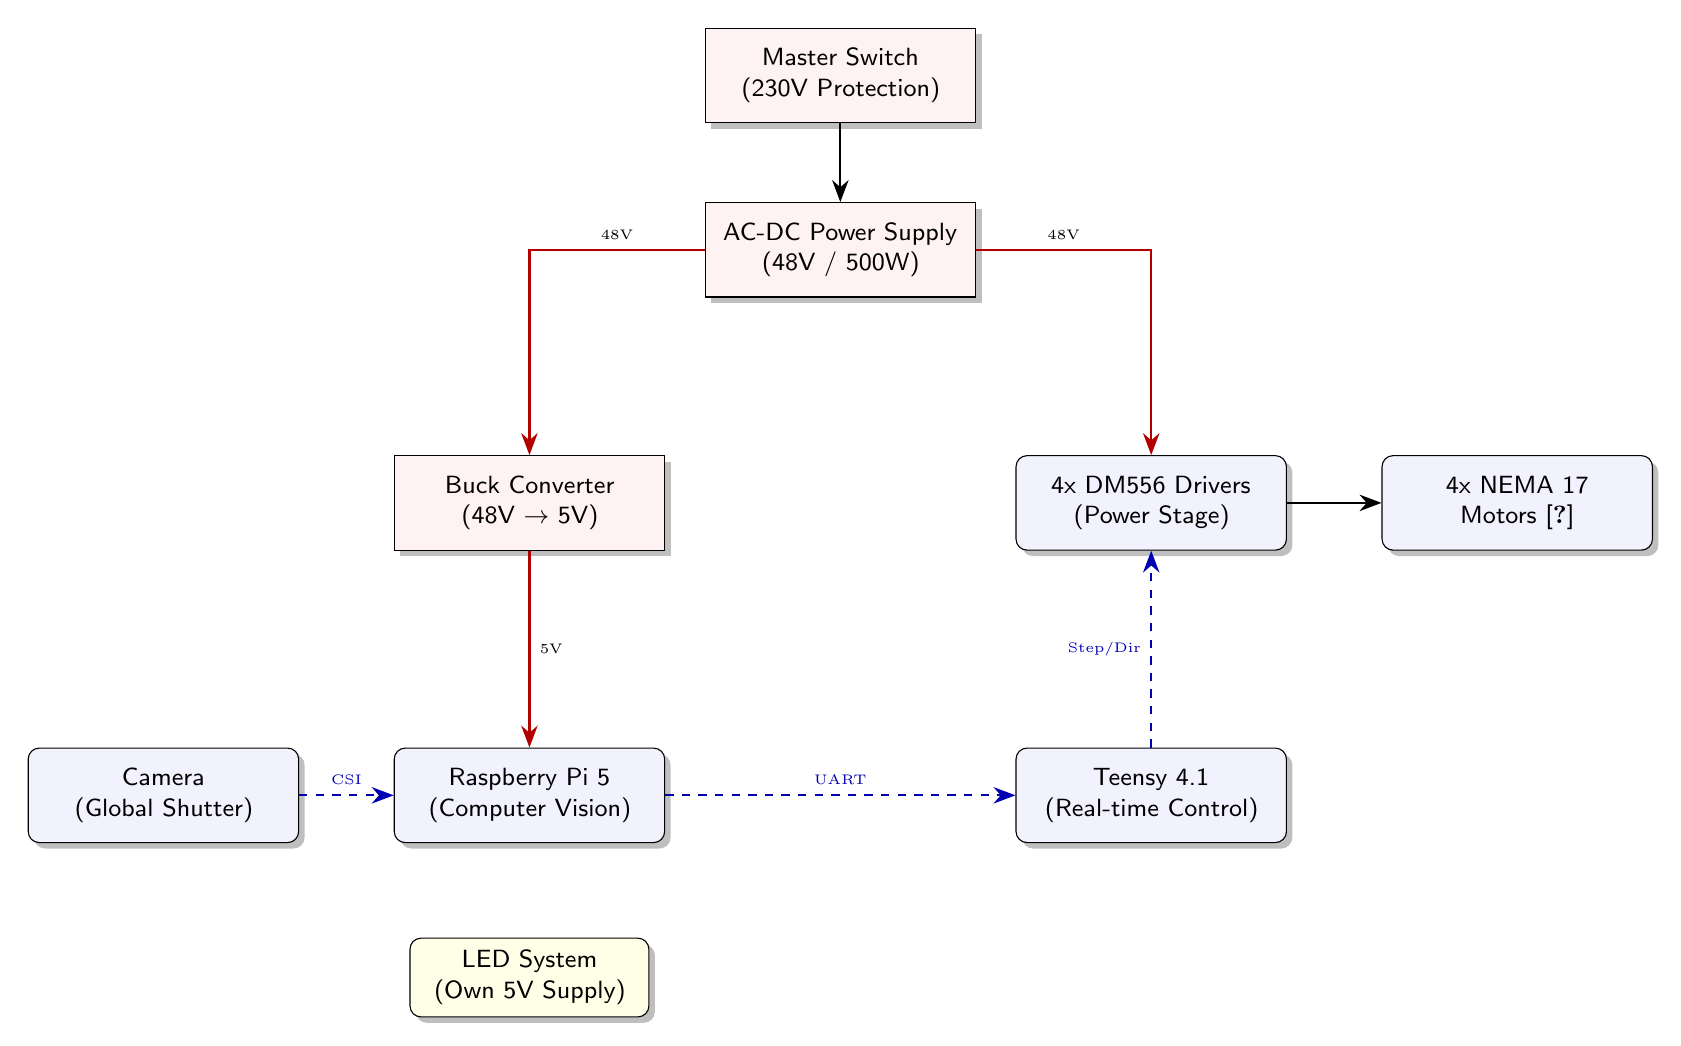
\begin{tikzpicture}[
    node distance=2cm and 1.5cm,
    block/.style={rectangle, draw, fill=blue!5, text width=3.2cm, text centered, rounded corners, minimum height=1.2cm, font=\small\sffamily, drop shadow},
    pwr/.style={rectangle, draw, fill=red!5, text width=3.2cm, text centered, minimum height=1.2cm, font=\small\sffamily, drop shadow},
    led/.style={rectangle, draw, fill=yellow!10, text width=2.8cm, text centered, rounded corners, minimum height=1cm, font=\small\sffamily, drop shadow},
    line/.style={draw, -{Stealth[scale=1.2]}, thick},
    pwrline/.style={draw, -{Stealth[scale=1.2]}, red!70!black, thick},
    dataline/.style={draw, -{Stealth[scale=1.2]}, blue!70!black, thick, dashed}
]

\node (psu) [pwr] {AC-DC Power Supply\\(48V / 500W)};
\node (switch) [pwr, above=1cm of psu] {Master Switch\\(230V Protection)};
\node (buck) [pwr, below left=2cm and 0.5cm of psu] {Buck Converter\\(48V $\to$ 5V)};
\node (drivers) [block, below right=2cm and 0.5cm of psu] {4x DM556 Drivers\\(Power Stage)};
\node (pi) [block, below=2.5cm of buck] {Raspberry Pi 5\\(Computer Vision)};
\node (teensy) [block] at (pi -| drivers) {Teensy 4.1\\(Real-time Control)};
\node (cam) [block, left=1.2cm of pi] {Camera\\(Global Shutter)};
\node (led) [led, below=1.2cm of pi] {LED System\\(Own 5V Supply)};
\node (motors) [block, right=1.2cm of drivers] {4x NEMA 17\\Motors \cite{nema17}};

\draw [line] (switch) -- (psu);
\draw [pwrline] (psu) -| node[above, pos=0.25, font=\tiny, black] {48V} (buck);
\draw [pwrline] (psu) -| node[above, pos=0.25, font=\tiny, black] {48V} (drivers);
\draw [pwrline] (buck) -- node[right, font=\tiny, black] {5V} (pi);
\draw [dataline] (cam) -- node[above, font=\tiny] {CSI} (pi);
\draw [dataline] (pi) -- node[above, font=\tiny] {UART} (teensy);
\draw [dataline] (teensy) -- node[left, font=\tiny] {Step/Dir} (drivers);
\draw [line] (drivers) -- (motors);

\end{tikzpicture}
}
\caption{\textit{Block diagram of the system.}}
\label{fig:block_diagram_vfinal}
\end{figure}

\subsection{Power Management}
The main energy source is an efficient AC-DC unit, which provides a voltage of \textbf{48V}. This value was chosen to power the power stages of the 4 \textbf{DM556} drivers. The high voltage allows the stepper motors to reach high angular speeds and sudden accelerations, necessary for the ball's ``kick'' phase, overcoming the torque limitations that usually appear at lower voltages (12V or 24V).

To power the logic subsystems, a \textbf{Step-down} converter lowers the voltage from 48V to \textbf{5V}, in order to power the \textbf{Raspberry Pi 5} and the camera. The DM556 drivers have no separate logic supply: their control electronics are powered from the 48V input.

The \textbf{Teensy 4.1} (the main microcontroller) is supplied through its USB connection to the Raspberry Pi 5, which is also used to upload the firmware. The \textbf{LED lighting} has its own 5V step-down module, independent of the Raspberry Pi 5, and is always on.

From the standpoint of safety during operation, the system integrates a \textbf{high-power load switch} placed directly on the input from the power supply. This switch fulfills the role of a safety barrier, allowing the instant disconnection of the entire assembly in the event of a mechanical or electrical failure, thus preventing damage to critical components or mechanical self-destruction in the event of a software error.

\subsection{Actuation System and Motion Control}
The control of the 4 stepper motors is carried out through industrial \textbf{DM556} drivers, using \textbf{Step/Dir}. The motion is smoothed by configuring the drivers to a high \textbf{microstepping} regime (1/16, corresponding to 3200 steps/revolution). This high resolution eliminates mechanical vibrations, giving the platform millimeter-level precision in controlling the tilt plane.

Although the source code includes support for closed-loop feedback through magnetic encoders, the current version of the system uses open-loop control. The absence of encoders simplifies the wiring and reduces the computational latency, relying on the extremely stable frequency of the signal generated by the Teensy 4.1 to prevent step loss.

\subsection{Communication and Data Flow}
The interfacing between the two computing units is important for the best possible performance of the system:
\begin{itemize}
    \item \textbf{Camera interface:} The camera communicates with the Raspberry Pi 5 through the dedicated \textbf{CSI (Camera Serial Interface)} port, ensuring a high-bandwidth data transfer and zero latency in the GPU's processing buffer.
    \item \textbf{Host-to-Controller:} The Raspberry Pi 5 and the Teensy 4.1 communicate bidirectionally through the \textbf{UART} protocol at a speed of \textbf{115,200 baud}. To guarantee the correctness of the data in an environment with electrical noise induced by the motors, a \textbf{custom serial protocol} was implemented. It contains the ball's state vector (position and velocity on the 3 axes) in structured packets, validated through checksums, thus ensuring that no command is executed with corrupted data.
\end{itemize}

\subsection{Electrical Schematic and Pin Assignment}
\label{sec:schematic}

Figures~\ref{fig:schematic_power}--\ref{fig:schematic_drive} show the complete electrical schematic, drawn in KiCad. The pin numbers of the Raspberry Pi 5 are the physical pins of the 40-pin header; the pin numbers of the Teensy 4.1 are its digital pin numbers, as used in the firmware. The four motor channels are identical; the pins of each channel are given in Table~\ref{tab:pinout}.

\begin{figure}[H]
   \centering
   \includegraphics[width=0.95\textwidth, trim=37.5bp 533.8bp 860.9bp 66.3bp, clip]{schematic.pdf}
   \caption{\textit{Electrical schematic, part 1 of 4: power supply.}}
   \label{fig:schematic_power}
\end{figure}

\begin{figure}[H]
   \centering
   \includegraphics[width=\textwidth, trim=339.9bp 317.8bp 522.5bp 66.3bp, clip]{schematic.pdf}
   \caption{\textit{Electrical schematic, part 2 of 4: Raspberry Pi 5, camera and lighting.}}
   \label{fig:schematic_vision}
\end{figure}

\begin{figure}[H]
   \centering
   \includegraphics[width=0.75\textwidth, trim=671.1bp 458.2bp 320.9bp 66.3bp, clip]{schematic.pdf}
   \caption{\textit{Electrical schematic, part 3 of 4: Teensy 4.1.}}
   \label{fig:schematic_control}
\end{figure}

\begin{figure}[H]
   \centering
   \includegraphics[width=0.95\textwidth, trim=872.7bp 623.8bp 32.9bp 66.3bp, clip]{schematic.pdf}
   \caption{\textit{Electrical schematic, part 4 of 4: motor drive, channel M0. The channels M1--M3 are identical; their STEP and DIR pins are listed in Table~\ref{tab:pinout}.}}
   \label{fig:schematic_drive}
\end{figure}

\begin{table}[H]
\centering
\begin{tabularx}{\textwidth}{|l|>{\raggedright\arraybackslash}X|>{\raggedright\arraybackslash}X|>{\raggedright\arraybackslash}X|}
\hline
\textbf{Signal} & \textbf{From} & \textbf{To} & \textbf{Notes} \\ \hline
48V supply & PSU V+ / V$-$ & DM556 +V / GND (all four), step-down IN+ / IN$-$ & Power stage of the drivers \\ \hline
5V supply & Step-down OUT+ / OUT$-$ & Pi 5 pins 2, 4 (5V) / pin 6 (GND) & Bypasses the USB-C input of the Pi \\ \hline
UART TX & Pi 5 pin 8 (GPIO14, TXD) & Teensy pin 0 (RX1) & \texttt{/dev/ttyAMA0} $\rightarrow$ \texttt{Serial1}, 115,200 baud, 3.3V \\ \hline
UART RX & Pi 5 pin 10 (GPIO15, RXD) & Teensy pin 1 (TX1) & Direction: Teensy $\rightarrow$ Pi \\ \hline
Flash request & Pi 5 pin 16 (GPIO23) & Teensy PROGRAM & Puts the Teensy in bootloader mode \\ \hline
USB & Pi 5 USB-A & Teensy micro-USB & Only power source of the Teensy (5V), common ground, firmware upload \\ \hline
Camera & Pi 5 CSI port & Camera module & Ribbon cable \\ \hline
Lighting & Separate 5V step-down module & LED system & Independent of the Raspberry Pi 5, always on \\ \hline
STEP M0 / DIR M0 & Teensy pins 8 / 7 & DM556 M0 PUL+ / DIR+ & Motor M0, rear right \\ \hline
STEP M1 / DIR M1 & Teensy pins 4 / 3 & DM556 M1 PUL+ / DIR+ & Motor M1, front right \\ \hline
STEP M2 / DIR M2 & Teensy pins 6 / 5 & DM556 M2 PUL+ / DIR+ & Motor M2, front left \\ \hline
STEP M3 / DIR M3 & Teensy pins 10 / 9 & DM556 M3 PUL+ / DIR+ & Motor M3, rear left \\ \hline
Signal return & DM556 GND terminal & PUL$-$, DIR$-$ and ENA$-$ of each driver & Common-cathode wiring; the return reaches the Teensy ground through the common ground of the non-isolated step-down converter \\ \hline
Enable & -- & DM556 ENA+ & Not connected (ENA$-$ on GND): drivers always enabled \\ \hline
Motor phases & DM556 A+, A$-$, B+, B$-$ & Motor coil A, coil B & One driver per motor \\ \hline
\end{tabularx}
\caption{\textit{Pin assignment of the electrical connections.}}
\label{tab:pinout}
\end{table}

\subsection{Component Ratings}

Table~\ref{tab:ratings} lists the electrical ratings of the components. The DM556 values are taken from the manufacturer's manual \cite{dm556}, the Teensy 4.1 values from the PJRC specifications \cite{teensy41}, and the Raspberry Pi 5 values from the product brief \cite{rpi5}.

\begin{table}[H]
\centering
\begin{tabularx}{\textwidth}{|l|>{\raggedright\arraybackslash}X|>{\raggedright\arraybackslash}X|}
\hline
\textbf{Component} & \textbf{Rating} & \textbf{Use in the system} \\ \hline
AC-DC PSU & Output 48V DC, 500 W (max. 10.4 A) & Supplies the four drivers and the step-down converter \\ \hline
Master switch & 230V AC, 300 A, waterproof, ignition-protected & Disconnects the 230V AC input \\ \hline
Step-down converter & OEM EMG122 buck module: input 10--90V, output 1.5--60V (set to 5V), max. 6 A / 100 W, efficiency up to 97.5\,\% & Supplies the Raspberry Pi 5 (5 A recommended); non-isolated, so its input and output share the ground \\ \hline
Raspberry Pi 5 & 5V DC, 5 A recommended (27 W); GPIO 3.3V, not 5V tolerant & Image processing, UART master \\ \hline
Teensy 4.1 & 5V via USB, on-board 3.3V regulator; I/O 3.3V, not 5V tolerant & 200 Hz control loop, STEP/DIR generation \\ \hline
DM556 driver ($\times 4$) & Supply 20--50V DC; output 1.8--5.6 A peak, set to 2.7 A RMS (3.8 A peak) with the DIP switches; isolated logic inputs, 5V nominal & Microstepping 1/16 (3200 pulses/revolution) \\ \hline
NEMA 17 motor ($\times 4$) & Bipolar, $1.8^\circ$/step (200 steps/revolution), rated 1.5 A per phase, 5 mm shaft \cite{nema17} & Arm actuation \\ \hline
Camera & Raspberry Pi Global Shutter Camera (Sony IMX296 sensor) with fisheye lens, CSI, used at $640 \times 480$ and 60 fps & Ball detection \\ \hline
LED lighting & 5V, from its own step-down module & Constant illumination, always on \\ \hline
\end{tabularx}
\caption{\textit{Electrical ratings of the components.}}
\label{tab:ratings}
\end{table}

Three aspects of these ratings are relevant for the operation of the system:
\begin{itemize}
    \item \textbf{Supply voltage margin:} The 48V bus is close to the 50V maximum of the DM556 drivers. During fast deceleration the motors return energy to the bus, so the voltage can briefly rise above the nominal value; the margin of 2V should be kept in mind if the power supply is replaced.
    \item \textbf{Logic levels:} The optically isolated inputs of the DM556 are specified for 5V signals, while the Teensy 4.1 outputs 3.3V. In the current system they are connected directly; a 3.3V to 5V level shifter would restore the nominal input current of the optocouplers.
    \item \textbf{Raspberry Pi 5 supply through the GPIO header:} Because the Pi 5 is supplied through pins 2 and 4, it does not negotiate its power with a USB-C supply, and by default it limits the total current of its USB ports to 600 mA. This is sufficient for the Teensy 4.1, which is the only USB device.
\end{itemize}

\chapter{Mathematical and Kinematic Modeling}
\label{chap:cinematica}

The kinematic model of the \textbf{OctoBouncer} system has the role of establishing a precise correlation between the Cartesian coordinate space (the position and orientation of the platform) and the joint space (the rotation angles of the 4 stepper motors). For this project, we implemented an inverse kinematics model based on the geometry of parallel systems with 4 support points, using the mathematical basis specific to parallel robots \cite{parallel_robot}, derived from the architecture of the Stewart manipulator \cite{ik_stewart}.

\section{Geometric Parameters of the System}
In the geometric calculations, we used the following constant dimensions, determined through CAD design and direct measurements:
\begin{itemize}[leftmargin=1.5cm]
    \item \textbf{$L_1$ (98.1 mm):} Length of the arm fixed on the motor shaft.
    \item \textbf{$L_2$ (92.0 mm):} Length of the transmission rod (intermediate link).
    \item \textbf{$L_3$ (54.0 mm):} Vertical offset created by the joint under the platform.
    \item \textbf{$R_b$ (129.0 mm):} Radius of the fixed base (distance from the center to the motor axis).
    \item \textbf{$R_p$ (110.0 mm):} Radius of the mobile platform (distance from the center to the spherical joint).
    \item \textbf{$h_0$ (100.0 mm):} Neutral operating height of the platform.
\end{itemize}

\section{Inverse Kinematics Calculation}
The purpose of the algorithm is to determine the motor angle $\alpha_i$ for each arm $i \in \{0, 1, 2, 3\}$, starting from the orientation angles $\theta_{pitch}$ (pitch) and $\theta_{roll}$ (roll).

\subsection{Determining the Position of the Anchor Points}
Each motor is positioned at an angle $\gamma_i$ relative to the central axis, defined in the source code as:
\begin{equation}
    \gamma = \{225^\circ, 135^\circ, 45^\circ, 315^\circ\}
\end{equation}

For a given orientation of the platform, the vertical height $Z_i$ of each joint on the platform is calculated by projecting the tilt angles onto the radial geometry:
\begin{equation}
    Z_i = h_0 + R_p \cdot (\sin(\theta_{roll}) \cdot \cos(\gamma_i) + \sin(\theta_{pitch}) \cdot \sin(\gamma_i))
\end{equation}

Taking into account the length of the joint $L_3$, the vertical target for the transmission rod becomes $Z_{target} = Z_i - L_3$.

\subsection{Solving the Arm Geometry (Law of Cosines)}
Solving the inverse kinematics for parallel manipulators is done by decomposing the system into independent kinematic loops (closed-loop vector equations) \cite{parallel_robot}. The problem reduces to a triangle formed in the vertical plane of each motor. The radial distance between the point on the base and the one on the platform is constant in horizontal projection:
\begin{equation}
    X_{offset} = |R_b - R_p|
\end{equation}

The direct distance $D$ between the motor axis and the spherical joint on the platform is:
\begin{equation}
    D = \sqrt{X_{offset}^2 + Z_{target}^2}
\end{equation}

Applying the \textbf{Law of Cosines} in the triangle formed by $L_1, L_2$ and $D$, we obtain the interior angle $\beta$:
\begin{equation}
    \beta = \arccos\left(\frac{L_1^2 + D^2 - L_2^2}{2 \cdot L_1 \cdot D}\right)
\end{equation}

The final rotation angle of the motor, $\alpha_i$, is the sum of the base geometric angle and the correction $\beta$:
\begin{equation}
    \alpha_i = \arctan2(Z_{target}, X_{offset}) + \beta
\end{equation}

\section{Implementation in the Control Loop}
\label{sec:ik_linear}

The complete model above is implemented in the firmware (the \texttt{calculateArmAngle} function) and describes the geometry of the mechanism. In the current version of the real-time loop, however, it is not called: for the small tilts needed for balancing, the relation between the tilt of the platform and the rotation of each arm is close to linear, so the controller uses a \textbf{linear mixing} of the two tilt commands. The PID outputs $\theta_{pitch}$ and $\theta_{roll}$ (Chapter~\ref{chap:control}) are expressed directly in degrees of arm rotation, and each arm receives:
\begin{equation}
    \alpha_i = \alpha_h + \sigma_i^{p}\,\theta_{pitch} + \sigma_i^{r}\,\theta_{roll}
\end{equation}
with the signs $(\sigma_i^{p}, \sigma_i^{r})$ equal to $(+1,+1)$, $(-1,+1)$, $(-1,-1)$ and $(+1,-1)$ for the motors M0 (rear right), M1 (front right), M2 (front left) and M3 (rear left), where $\alpha_h$ is the common arm angle that sets the height of the platform (Section~\ref{sec:height_control}). A positive pitch command thus raises the rear arms and lowers the front ones, and a positive roll command raises the right side. All angles $\alpha_i$ are measured from the mechanical low stop of the arms. This simplification avoids the trigonometric calculations in the 200\,Hz loop; the gains of the PID controller absorb the constant ratio between arm rotation and platform tilt.

\section{Mechanical Limitations and Constraints}
For reasons of structural safety and to prevent collisions between links or the locking of joints (singularities), we implemented a strict software limitation of the tilt commands:
\begin{equation}
    -12^\circ \leq \theta_{pitch, roll} \leq 15^\circ
\end{equation}
In addition, every arm command is limited to the range $5^\circ \leq \alpha_i \leq 40^\circ$ above the low stop, so that the arms never press against the stop, and the common height angle $\alpha_h$ is kept at $17^\circ$ or more, which leaves $12^\circ$ of tilt range below; upwards it is only bounded by the $40^\circ$ arm limit. With only $10^\circ$ below (the earlier setting), the lower arm reached its limit as soon as pitch and roll together asked for more than $10^\circ$, and stopped reacting; an upper height limit of $30^\circ$ (also removed after the tests) stopped the height control while the plate still had to rise.

These constraints keep the system in a zone of relative linearity and prevent the motors from being forced into extreme positions. At the moment, the \textit{bouncing} function is disabled. As shown below, the limiting factor is not the strength of the PET-G structure, but the torque of the directly driven stepper motors: an acceleration high enough to throw the ball would make them lose steps, and since the system works in open loop, every lost step remains as an offset of the plate height and tilt.

\subsection{Maximum Vertical Acceleration}
\label{sec:max_accel}

The vertical acceleration of the platform is bounded by the force that the four arms can apply. A motor torque $\tau$ acting on the arm of length $L_1$ produces at most a vertical force $\tau / L_1$ at its end (when the arm is horizontal), so the upward acceleration of the moving mass $m$ is limited to:
\begin{equation}
    a_{max} = \frac{4\,\tau / L_1 - m\,g}{m}
\end{equation}
The moving mass is dominated by the 8\,mm plexiglass plate (an octagon with flat edges 110\,mm from its center, about 401\,cm$^2$ and 0.38\,kg at 1.19\,g/cm$^3$); with the upper joints and rods we take $m \approx 0.45$\,kg. For the holding torque of the NEMA 17 motors we use 0.4\,Nm, a typical value for this motor class (the supplier gives no value) \cite{nema17}. Because a stepper motor loses steps well before its holding torque is reached, especially while the same motors also control the tilt, only about half of it can be used safely.

\begin{table}[H]
\centering
\begin{tabularx}{\textwidth}{|>{\raggedright\arraybackslash}X|c|c|c|}
\hline
\textbf{Drive} & \textbf{Torque at the arm [Nm]} & \textbf{Force, 4 arms [N]} & \textbf{$a_{max}$ [m/s$^2$]} \\ \hline
Direct, holding torque & 0.40 & 16.3 & 26.4 (2.7\,g) \\ \hline
Direct, usable (50\,\%) & 0.20 & 8.2 & \textbf{8.3 (0.85\,g)} \\ \hline
5:1 gearbox (90\,\% efficiency), usable & 0.90 & 36.7 & 71.7 (7.3\,g) \\ \hline
\end{tabularx}
\caption{\textit{Maximum upward acceleration of the platform ($m \approx 0.45$\,kg, $L_1 = 98.1$\,mm), in addition to the acceleration of gravity.}}
\label{tab:max_accel}
\end{table}

To throw the ball to a height $h$, the plate has to reach the speed $v = \sqrt{2gh}$ and then stop faster than the ball falls back. Over a stroke of 10\,mm, which the arm range allows around the working height, this requires an acceleration of $v^2 / (2 \cdot 10\,\text{mm})$: about 1\,g for a 1\,cm bounce, 2\,g for 2\,cm and 5\,g for 5\,cm. With the direct drive, the \textbf{maximum safe vertical acceleration is therefore about 8\,m/s$^2$ (0.85\,g)}, below what even a 1\,cm bounce needs. A 5:1 gearbox raises the usable acceleration to about 7\,g, enough for bounces of several centimeters; the arm speed needed for a 5\,cm bounce (about 96\,rpm, i.e.\ 480\,rpm at the motor) remains within the range of such gearboxes. Gearboxes are therefore planned for the next version of the system.

The PET-G arms are not the limit, because the load they carry cannot exceed the torque of the motor that drives them: a larger load stalls the motor instead. The largest bending moment in an arm is thus 0.4\,Nm with the direct drive and about 1.8\,Nm with a 5:1 gearbox. PET-G filament has a tensile strength of about 50\,MPa along the extrusion direction, and printed parts are weaker across their layers \cite{petg_material}; with a conservative allowable stress of 20\,MPa, the arm needs a section modulus of only 20\,mm$^3$ (direct drive) or 90\,mm$^3$ (gearbox), i.e.\ a solid rectangular section of about $3 \times 6$\,mm or $5 \times 10$\,mm. Each arm (98.1\,mm from the motor shaft to the joint of the rod) is built from 3\,mm plates, 25\,mm wide, always used in pairs: two stacked plates are fixed to the motor hub, two further plates enclose them from both sides and are clamped to them by two bolts, and continue as a pair to the joint, where the rod (itself two stacked plates with the bearing) is attached. The arm is therefore 6\,mm thick next to the hub and at the joint, and 12\,mm where the plates overlap. The critical section is next to the motor hub, where the bending moment is largest: $6 \times 25$\,mm bent in its own plane, i.e.\ a section modulus of 625\,mm$^3$. There the stress is 0.6\,MPa with the direct drive and 2.7\,MPa with a 5:1 gearbox: a safety factor of 34 and 7.6 against the conservative 20\,MPa, and of about 85 and 19 against the strength along the extrusion direction, along which the flat-printed plates are loaded. The most loaded point is the connection to the aluminum motor hub, whose four M3 screws on a 12.7\,mm circle transmit the torque: each one presses on its hole in the two plates with 16\,N (bearing stress 0.75\,MPa) with the direct drive and with 71\,N (3.4\,MPa, safety factor 5.9) with the gearbox. The two bolts that clamp the plates carry less (at most about 55\,N, 2.2\,MPa, with the gearbox). The impact of the ball itself (2.7\,g) is negligible. What remains to be verified with gearboxes is the long-term behavior of the printed parts under repeated impulses: fatigue at the screw holes of the hub and at the bearing seats, and the strength of the layer bonds.

\chapter{Control Strategy}
\label{chap:control}

The control system of the \textbf{OctoBouncer} is distributed between two processing units, the final goal being to keep the ball in the center of the platform (or to follow a trajectory) by continuously adjusting the tilt plane.

\section{Distributed Control Architecture}
To maximize performance, we separated the processing tasks into two levels:
\begin{enumerate}
    \item \textbf{High Level:} The Raspberry Pi 5 runs the image processing algorithms under OpenCV, extracting the $(x, y)$ coordinates of the ball and calculating the velocity vectors $(V_x, V_y)$ at a high frequency.
    \item \textbf{Execution Level:} The Teensy 4.1 receives the data through UART and runs the PID control loop at a frequency of \textbf{200 Hz} (5 ms), generating the Step/Dir signals for the motors.
\end{enumerate}

\section{PID Control Algorithm}
The core of the stabilization is a \textbf{Proportional-Integral-Derivative (PID)} controller \cite{pid_control}. The calculation formula for the desired tilt angle (on each axis) is:
\begin{equation}
    \theta(t) = K_p \cdot e(t) + K_i \cdot \int_{0}^{t} e(\tau) d\tau + K_d \cdot \left(V_{ball}(t) - V_{target}(t)\right)
\end{equation}
where $e(t)$ is the difference between the filtered position of the ball and the target position.

Where the components fulfill the following roles:
\begin{itemize}
    \item \textbf{Proportional Term ($K_p$):} Reacts instantaneously to the ball's position error relative to the target (the center of the platform or the current point of the trajectory).
    \item \textbf{Integral Term ($K_i$):} Eliminates steady-state errors caused by possible mechanical imperfections or residual tilts of the base. We implemented an \textit{anti-windup} limitation of the integral to prevent saturation of the integrator.
    \item \textbf{Derivative Term ($K_d$):} Acts as a ``brake'' (damping). The velocities of the ball and of the target are estimated on the Teensy by differentiating their EMA-filtered positions (Section~\ref{sec:ema}) and smoothing the result with a second EMA filter ($\alpha = 0.2$), which attenuates the numerical noise of the differentiation \cite{derivative_filter}. The term acts on the velocity of the ball \textit{relative to the target}: a ball that moves together with a moving target is not braked, while with a fixed target (CENTER mode) the term reduces to a derivative on the measurement, which avoids command jumps when the target changes. The velocity estimated by the Raspberry Pi is also transmitted, but is not used by the controller. Section~\ref{sec:exp_before_after} compares this form with a derivative acting on the ball's own velocity.
\end{itemize}

\section{Real-Time Image Processing Subsystem (Raspberry Pi)}
\label{sec:vision}

The high level of the control architecture is implemented as a Python script running continuously on the \textbf{Raspberry Pi 5}, which can be launched automatically at startup. Its responsibility is to transform the stream of frames from the camera into a complete state vector of the ball, made up of three-dimensional position and velocities, transmitted in real time to the Teensy 4.1. The subsystem code is organized modularly, each script fulfilling a distinct role in the development and operation flow of the system.

\subsection{Camera Calibration with Fisheye Lens}

The camera used is a \textbf{Raspberry Pi Global Shutter Camera}: its sensor exposes all pixels at the same time, so a fast-moving ball is not distorted as with a rolling shutter. It is equipped with a \textbf{fisheye (ultra-wide angle)} lens, which, although it maximizes the field of view in order to cover the entire surface of the platform, introduces a pronounced radial distortion. Straight lines appear curved, and objects at the edge of the frame are scaled non-uniformly relative to the center. Using raw pixel coordinates in the position calculations would introduce unacceptable systematic errors into the control loop.

The calibration process takes place in two steps implemented in the \texttt{camera\_calib} module:

\begin{enumerate}
    \item \textbf{Capturing the calibration images (\texttt{1\_capture\_images.py}):} A checkerboard pattern with a grid of $9 \times 7$ squares ($8 \times 6$ interior corners) is used. The operator presents the board in front of the camera at various angles and distances, saving one frame at each press of the \texttt{'s'} key, at the moment when the \texttt{findChessboardCorners} algorithm \cite{chessboard_corners} visually confirms the complete detection. The calibration set used comprises 31 images, covering sufficient spatial variations to characterize the distortion across the entire sensor area.

    \item \textbf{Calculating the intrinsic parameters (\texttt{2\_calibrate\_calc.py}):} Based on the set of images, the \texttt{cv2.fisheye.calibrate} algorithm from OpenCV \cite{opencv_calib} is run, which determines the camera's intrinsic matrix $\mathbf{K}$ and the fisheye distortion vector \cite{fisheye_calib, opencv_remap} $\mathbf{D}$ (with 4 coefficients). The correction of the corners is carried out through \texttt{cornerSubPix} to a precision of $0.001$ pixels. The resulting parameters are saved in a binary Numpy array file, \texttt{cam\_calib\_fisheye.npz}, loaded at every system startup.
\end{enumerate}

Based on these parameters, two rectification tables (\texttt{map1}, \texttt{map2}) are generated through the \texttt{cv2.fisheye.initUndistortRectifyMap} function. The \texttt{cv2.remap} function applies a bilinear rectification on each captured frame, efficiently transforming the initial fisheye projection into a distortion-free plane-perspective image. The parameter \texttt{balance = 1.0} ensures that the entire field of view is preserved without cropping, at the cost of some black edges at the corners.

\subsection{Ball Color Calibration (\texttt{1\_tune\_color.py})}

The detection of the ball is based on color segmentation in the \textbf{HSV} space \cite{hsv_seg}, chosen instead of RGB for decoupling the hue information from lighting variations. Before the first use, or whenever the ball, the light source or the ambient environment changes, the interactive color calibration script must be run.

The graphical interface exposes six sliders, corresponding to the lower thresholds $[H_{min}, S_{min}, V_{min}]$ and to the upper thresholds $[H_{max}, S_{max}, V_{max}]$. The values are adjusted in real time while simultaneously observing the original image and the resulting binary mask, with the aim of maximizing the white area corresponding to the ball and eliminating any false positives from the background. The camera is configured in \textbf{manual} mode (without auto-exposure and without automatic white balance), with the exposure time set to \textbf{20\,ms} (limited by the camera to the frame period of 16.7\,ms at 60\,fps) and the analog gain at \textbf{2.0}. Upon pressing the \texttt{'q'} key, the calibrated values are saved in the \texttt{hsv\_values.txt} file and will be loaded automatically at subsequent startups.

\begin{figure}[H]
   \centering
   \includegraphics[width=\textwidth]{color_calib.png}
   \caption{\textit{The HSV calibration interface: the original window (left), the slider panel with the current thresholds (center) and the resulting binary mask - the ball appears white, the background black (right).}}
\end{figure}

\subsection{Processing Pipeline and State Estimation}

The main processing loop, implemented in \texttt{4\_headless\_track.py} (without display, for autonomous operation) and \texttt{4\_gui\_track.py} (with display, for monitoring and diagnostics), successively goes through the stages described below at an acquisition frequency of \textbf{60 fps}, a resolution of $640 \times 480$ pixels, through the dedicated \textbf{CSI} interface of the Raspberry Pi 5.

\begin{enumerate}
    \item \textbf{Capture and geometric correction:} The BGR frame is captured directly through the \texttt{Picamera2} library \cite{picamera2} in native format, avoiding an additional color conversion. The precomputed fisheye rectification is applied immediately.

    \item \textbf{HSV segmentation and morphological operations:} The corrected image is converted into the HSV space, and the binary mask is obtained through a color threshold. An \textbf{erosion} followed by a \textbf{dilation} with a $3 \times 3$ kernel is applied to the mask, eliminating point artifacts without affecting the geometry of the ball.

    \item \textbf{Contour selection and radius estimation:} The \texttt{cv2.findContours} function extracts all the connected regions from the mask. The contour with the maximum area is selected as the sole candidate. The \texttt{cv2.minEnclosingCircle} function determines the center $(x_{px}, y_{px})$ and the radius $r_{px}$ in pixels. A minimum threshold filter $r_{px} > 5$ eliminates false detections caused by reflections or other surrounding objects with similar hues.

    \item \textbf{3D reconstruction through the corrected pinhole model:} The depth $Z$ is estimated from the apparent diameter of the ball in the geometrically corrected image, using an extended pinhole model with angular correction to compensate for the perspective elongation effect at the edges of the image:
    \begin{equation}
        Z_{pinhole} = \frac{f_x \cdot D_{real}}{2 \cdot r_{px}}, \quad
        Z_{final} = Z_{pinhole} \cdot \sqrt{1 + \left(\frac{d_{center}}{f_x}\right)^2}
    \end{equation}
    where $D_{real} = 40\,\text{mm}$ is the real diameter of the ball, $f_x$ is the focal length extracted from the new camera matrix $\mathbf{K'}$, and $d_{center}$ is the distance in pixels from the optical center. The planar coordinates in millimeters are calculated through inverse projection:
    \begin{equation}
        X_{real} = \frac{(x_{px} - c_x) \cdot Z_{final}}{f_x}, \quad Y_{real} = \frac{(y_{px} - c_y) \cdot Z_{final}}{f_y}
    \end{equation}

    \item \textbf{Plate-centered coordinates:} The positions are finally expressed relative to the center of the plate, which lies $(8.0, -1.2)$\,mm from the optical center of the camera (measured once from markers on the brackets, with the plate level). The CENTER target and all patterns are therefore centered on the plate.

    \item \textbf{Median filtering of the depth:} Because $X_{real}$ and $Y_{real}$ are proportional to $Z_{final}$, a single-frame error in the estimated radius would move the ball position and produce a false velocity. The depth is therefore passed through a \textbf{median filter}: the median of the last 15 frames (0.25\,s) is used to scale $X$ and $Y$, and the median of the last 5 frames is reported as $Z$. The median removes isolated outliers without smoothing real movements as strongly as an average.
\end{enumerate}

\subsection{Velocity Estimation and Two-Stage Filtering}

Since the velocity of the ball cannot be obtained through direct measurement, it is estimated numerically. Differentiating the positions between consecutive frames amplifies the quantization errors, requiring a two-level filtering for noise attenuation:

\begin{enumerate}
    \item \textbf{Filtering the raw position (EMA with $\alpha_{pos} = 0.6$):} Before computing the derivative, the raw positions are filtered. A higher $\alpha$ means that the system tracks the ball quickly, but passes more noise to the velocity estimation.

    \item \textbf{Filtering the calculated velocity (EMA with $\alpha_{vel} = 0.15$):} The resulting numerical velocity is passed through an aggressive low-pass filter. The value $\alpha_{vel} = 0.15$ was determined experimentally: higher values ($> 0.4$) leave residual vibrations that destabilize the derivative term of the PID, while lower values ($< 0.05$) introduce a noticeable phase delay at sudden changes of direction.
\end{enumerate}

These velocities are displayed in the diagnostic interface and transmitted to the Teensy, which computes its own estimate for the controller (Chapter~\ref{chap:control}). An additional \textbf{deadband} mechanism ($1.5\,\text{mm}$) treats displacements that are below the threshold as null, eliminating false velocities under stationary-ball conditions. If the ball disappears from the field of view, the velocity is decremented exponentially (factor $0.8$ per frame) instead of being reset abruptly, preventing command shocks at re-detection.

\subsection{Tuning Parameters}

The optimal functioning of the frame capture and processing subsystem depends on the correct calibration of the parameters grouped in the following table. They are adjustable both by directly modifying the source files and at runtime through the dedicated graphical interfaces.

\begin{table}[H]
\centering
\begin{tabularx}{\textwidth}{|X|X|X|}
\hline
\textbf{Parameter} & \textbf{Current value} & \textbf{Impact when adjusted} \\ \hline
$[H_{min}, S_{min}, V_{min}]$ & $[98, 145, 40]$ & Too narrow: detection losses; too wide: false positives from the environment \\ \hline
$[H_{max}, S_{max}, V_{max}]$ & $[116, 255, 255]$ & Upper limit of the accepted color; $S_{max}$ and $V_{max}$ at 255 include the entire brightness range \\ \hline
$r_{px,min}$ (minimum radius) & $5\,\text{px}$ & Below this value, the detection is ignored; prevents false positives from reflections \\ \hline
$\alpha_{pos}$ (position EMA) & $0.6$ & Higher values: fast tracking, but more noise toward the velocity estimator \\ \hline
$\alpha_{vel}$ (velocity EMA) & $0.15$ & Compromise between attenuating the derivative noise and the response latency at impact \\ \hline
\textit{Deadband} & $1.5\,\text{mm}$ & Eliminates velocity drift at rest; too large masks real slow movements \\ \hline
\texttt{balance} (undistort) & $1.0$ & $0.0$ = central crop without black edges; $1.0$ = maximum field of view preserved \\ \hline
\end{tabularx}
\caption{\textit{Configuration parameters of the visual detection subsystem and their effect on the behavior of the system.}}
\end{table}

\subsection{Live Visualization and Diagnostic Interface}

The versions with display (\texttt{4\_gui\_track.py}, \texttt{4\_gui\_track\_w\_mode.py}) overlay a diagnostic layer on top of the corrected video stream, intended exclusively for tuning and debugging. The overlay displays the ball detection status (FOUND/LOST), the spatial coordinates $(X, Y, Z)$ and the velocities $(V_x, V_y, V_z)$ in real time, the green circle superimposed on the detected ball, the current operating mode of the system, as well as a real-time animation in the bottom-right corner.

\begin{figure}[H]
   \centering
   \includegraphics[width=0.75\textwidth]{center_mode.png}
   \caption{\textit{The GUI interface in CENTER mode: the ball is kept in the center of the platform, and the minimap indicates the target position (green) relative to the actual position of the ball (yellow).}}
\end{figure}

\subsection{Trajectory Generator and Pattern Selection}

In addition to stabilization at a fixed point, the \textbf{OctoBouncer} system implements a trajectory generator that forces the ball to follow predefined geometric shapes. The active mode is controlled bidirectionally through the UART protocol: the Teensy 4.1 notifies the Raspberry Pi at each pattern transition, and the user can change the mode from the graphical interface by pressing the keys \texttt{1}--\texttt{5}, without any need for a direct modification in the code.

Four distinct trajectories are defined, plus an automatic cycling mode:

\begin{itemize}
    \item \textbf{CENTER (key 1):} The ball is kept at the origin of the platform. The target is fixed at $(0, 0)$.
    \item \textbf{CIRCLE (key 2):} The ball follows a circular trajectory with a radius of 50\,mm and a period of 5\,s.
    \item \textbf{STAR (key 3):} A 5-pointed star-shaped trajectory, alternating between the outer radius of 60\,mm and the inner one of 25\,mm, with a period of 10\,s.
    \item \textbf{FIGURE 8 (key 4):} A figure-eight-type trajectory (lemniscate), with a horizontal semi-axis of 60\,mm and a vertical one of 30\,mm, with a period of 6\,s.
    \item \textbf{CYCLE ALL (key 5):} The system automatically cycles through all four modes above, 25\,s each, with smooth transitions ensured by a target rate limiter of 120\,mm/s.
\end{itemize}

Two further patterns, \textbf{STEP X} and \textbf{STEP Y}, are used only by the automated test protocol (Chapter~\ref{chap:rezultate}): the target jumps between $-30$ and $+30$\,mm along one axis every 8\,s, through the same rate limiter.

The synchronization of the visualization with the real execution is ensured by transmitting the current target position $(t_x, t_y)$ from the Teensy to the Raspberry Pi through a dedicated \texttt{PACKET\_TYPE\_TARGET\_POS} packet at every 5\,ms iteration. Thus, the green dot in the animation reflects exactly the coordinate followed by the PID controller.

\begin{figure}[H]
    \centering
    \begin{minipage}{0.32\textwidth}
        \centering
        \includegraphics[width=\textwidth]{circle_mode.png}
        \caption{\textit{CIRCLE mode.}}
    \end{minipage}\hfill
    \begin{minipage}{0.32\textwidth}
        \centering
        \includegraphics[width=\textwidth]{star_mode.png}
        \caption{\textit{STAR mode.}}
    \end{minipage}\hfill
    \begin{minipage}{0.32\textwidth}
        \centering
        \includegraphics[width=\textwidth]{figure_eight_mode.png}
        \caption{\textit{FIG8 mode.}}
    \end{minipage}
\end{figure}

\subsection{Real-Time PID Tuning Interface}

The \texttt{4\_gui\_track\_pid.py} script extends the diagnostic interface with three sliders that allow adjusting the coefficients $K_p$, $K_i$ and $K_d$ in real time, without restarting the system. The sliders start from the default values hardcoded in the firmware ($K_p = 0.149$, $K_i = 0.112$, $K_d = 0.068$, for positions expressed in the units of the HSV pipeline; see Section~\ref{sec:exp_method}). The values are scaled internally by the factor $\frac{1}{1000}$ and are transmitted to the Teensy through a dedicated packet of type \texttt{PACKET\_TYPE\_PID\_UPDATE} once the user modifies any slider. The current coefficients are also displayed in the video overlay (in light green, under the velocities section).

\begin{figure}[H]
   \centering
   \includegraphics[width=0.75\textwidth]{pid_calib.png}
   \caption{\textit{The PID tuning interface: the P, I, D sliders visible in the lower part of the window, with the current values displayed in the overlay (light green). Pattern selection remains available through the keys 1--5.}}
\end{figure}

\subsection{Serial Communication Protocol}

At the end of each processing cycle, the ball's state vector is serialized and transmitted through \textbf{UART} at \textbf{115,200 baud}. The implemented custom protocol has the structure:

\begin{equation}
    \underbrace{\texttt{0xAA}}_{\text{start}} \;|\; \underbrace{\texttt{TYPE}}_{\text{packet type}} \;|\; \underbrace{\texttt{SIZE}}_{\text{length}} \;|\; \underbrace{\texttt{PAYLOAD}}_{\text{data}} \;|\; \underbrace{\texttt{CSUM}}_{\text{XOR}} \;|\; \underbrace{\texttt{0xBB}}_{\text{stop}}
\end{equation}

The checksum is calculated as an accumulated XOR over the packet type, the size and each byte of the payload. The checksum is validated on the Teensy before the data is introduced into the PID loop; a corrupted packet is ignored, and the system continues with the last valid state. Five packet types are defined: \texttt{BALL\_DATA} (the positions $X, Y, Z$ and the velocities $V_x, V_y, V_z$ packed as 6 32-bit floats, with a status byte \texttt{is\_found}), \texttt{PID\_UPDATE} (three floats with the new coefficients), \texttt{START} (initialization signal), \texttt{PATTERN\_CHANGE} (mode change, bidirectional) and \texttt{TARGET\_POS} (the current target position and the height setting of the platform, transmitted by the Teensy to the Pi at every 5\,ms iteration for the synchronization of the minimap). The Teensy reads only the position and the detection status from \texttt{BALL\_DATA}.

\section{Data Filtering (EMA Filter)}
\label{sec:ema}
The received position data may exhibit white noise due to the camera resolution or lighting variations. To normalize the system's response without introducing significant latencies, we used an \textbf{EMA (Exponential Moving Average)} filter \cite{ema_filter}:
\begin{equation}
    X_{filtrat} = \alpha \cdot X_{raw} + (1 - \alpha) \cdot X_{anterior}
\end{equation}
The value $\alpha = 0.15$ was chosen experimentally to balance noise attenuation with the reaction speed of the system. The target position is passed through an identical filter before its velocity is computed, so that the two velocities compared in the derivative term have the same delay.

\section{Real-Time Management and Synchronization}
The stability of a ``Ball and Plate'' system depends on the constancy of the sampling period. The Teensy 4.1 uses a high-precision internal clock to ensure the execution of the control loop at exactly 5 ms. The firmware is written in C++ and built with PlatformIO \cite{platformio}.
\begin{itemize}
    \item If the data from the Raspberry Pi is delayed, the system uses the last known state to maintain stability.
    \item The motor movement is interpolated to avoid mechanical shocks, ensuring a smooth transition between the calculation steps of the PID.
\end{itemize}

\section{Safety Limitations (Software Constraints)}
To protect the mechanical structure, the angles calculated by the PID are passed through a limiting block before being converted into arm commands (Section~\ref{sec:ik_linear}), and every arm command is limited to its safe range. This prevents reaching the mechanical limits of the joints in the case of violent movements or if the ball accidentally leaves the platform.

An \textbf{edge guard} protects the ball itself: when it moves more than 85\,mm from the center of the plate, close to the edge and to the screws of the brackets, the target is moved back to the center (through the rate limiter) until the ball is again within 40\,mm; then the pattern continues.

\section{Plate Height Control}
\label{sec:height_control}

The arm angles are measured from the mechanical low stop, so the arms must rest on the stop when the Raspberry Pi sends the \texttt{START} command. At startup the Teensy lifts all arms to $5^\circ$ in 1\,s, then raises them together at $2^\circ$/s to $17^\circ$ while the balancing loop is already active, so the ball can be placed on the platform immediately.

From there, the common height angle $\alpha_h$ is controlled from the measured depth of the ball: since the camera is under the platform, a higher platform increases $Z$. The Teensy keeps the ball at $Z = 195 \pm 4$\,mm by moving $\alpha_h$ at $0.05^\circ$/s per millimeter of error, at most $2^\circ$/s, between $17^\circ$ and the $40^\circ$ arm limit. The depth is low-pass filtered and only used while the ball is within 75\,mm of the center, where its estimate is reliable. The height setting is reported to the Raspberry Pi in the \texttt{TARGET\_POS} packet.

\chapter{Experimental Results and Conclusions}
\label{chap:rezultate}

\section{Experimental Method}
\label{sec:exp_method}

We measured the performance of the \textbf{OctoBouncer} on the physical system in two test runs. Both use the final control configuration: \textbf{median-filtered depth}, a \textbf{derivative term acting on the velocity of the ball relative to the target}, and \textbf{closed-loop control of the plate height}.

\begin{itemize}
    \item \textbf{Run A (24 October 2026):} four runs (runs 7--10) in the automatic cycling mode (\textbf{CYCLE ALL}), in which the controller follows each pattern for 25\,s: CENTER, CIRCLE, STAR and FIGURE 8. The ball was placed on the plate at start-up and the system was not touched afterwards. A fifth run (run 1), recorded with the same vision system but before the control changes (derivative term on the ball's own velocity, depth not filtered), serves as the reference for the comparison of the two derivative terms in Section~\ref{sec:exp_before_after}.
    \item \textbf{Run B (25 October 2026):} an automated test protocol (\texttt{5\_test\_runner.py}) ran five times in a row, 42.6\,min and 153{,}380 frames at 60\,fps in total. Each run consists of 60\,s in CENTER, 64\,s of target steps along each axis (Section~\ref{sec:exp_steps}), 60\,s of each pattern and five light taps on the ball held in CENTER (Section~\ref{sec:exp_disturb}). Every test starts from the ball at rest after 10\,s in CENTER, so all transitions are the same. The ball fell off once and was put back; the interrupted phase was repeated automatically.
\end{itemize}

Run B differs from run A in three details, introduced between the two: the positions are relative to the center of the plate instead of the camera (Section~\ref{sec:vision}), the edge guard is active, and the tilt range is that of Section~\ref{sec:ik_linear} (in run A: $-10^\circ$ to $15^\circ$, and a minimum height of $15^\circ$). In both runs the plate height was still limited to $30^\circ$. Only the final derivative term was tested in run B.

In these runs the ball positions are expressed in true millimeters. The HSV pipeline of Section~\ref{sec:vision} reports about $1/1.4$ of the true distances, because the dilated mask overestimates the apparent radius of the ball; the PID gains of Chapter~\ref{chap:control} were therefore divided by the same factor 1.4, so that the controller behaves identically.

For every camera frame (\textbf{60 Hz}) the tracking script on the Raspberry Pi 5 logs the measured ball position $\mathbf{p}_{ball}(t)$ and the target $\mathbf{p}_{target}(t)$ that the Teensy 4.1 reports through the \texttt{TARGET\_POS} packet every 5\,ms, i.e.\ exactly the set-point used by the PID controller. All coordinates are in millimeters, relative to the camera's optical center in run A and to the center of the plate in run B. In run B every frame also carries its exposure time (the camera's \texttt{SensorTimestamp}); the ball position is evaluated at that instant and the target is interpolated to it, so the delay between exposure and processing (25.3\,ms, median) does not appear as lag. The tracking error is defined as:
\begin{equation}
    e(t) = \lVert \mathbf{p}_{ball}(t) - \mathbf{p}_{target}(t) \rVert
\end{equation}

The following quantities were computed for each pattern phase:
\begin{itemize}
    \item \textbf{Steady-state error:} The mean, RMS, 95th percentile (P95) and maximum of $e(t)$ over the last 15\,s of each 25\,s phase. The final 0.5\,s of each phase are excluded, because the target already moves towards the next pattern.
    \item \textbf{Settling time ($t_s$):} The time after the pattern switch from which the 1\,s moving RMS of $e(t)$ stays below $1.1$ times the largest 1\,s moving RMS observed in the steady-state window. A value of zero means that the switch produced no error transient larger than the pattern's own steady-state error.
    \item \textbf{Lag:} The time shift of the measured path that minimizes its mean squared distance to the target (positive: the ball is behind the target; negative: ahead of it).
    \item \textbf{Shape deviation and amplitude ratio:} The mean distance of the measured path from the ideal curve, and the ratio between the ball's mean distance from the center and the target's.
    \item \textbf{Step response} (run B): for each 60\,mm step, the rise time from 10 to 90\,\% of the step, the delay between the 50\,\% points of target and ball, the overshoot, and the settling time to $\pm$5\,\% of the step (3\,mm) and to $\pm$2\,mm, measured from the start of the target ramp.
    \item \textbf{Disturbance rejection} (run B): the largest distance of the ball from the center after a tap, and the time until it stays within 5\,mm of the center for at least 1\,s.
\end{itemize}

In run B the steady state of the patterns is the window from 20 to 60\,s after the start, and CENTER is evaluated from 5\,s after the start.

Two checks support the validity of the measurement. First, the commanded target coincides with the mathematical trajectories of Section~\ref{sec:exp_traj} (maximum deviation $0.07$\,mm), so the target rate limiter is not active in steady state and the comparison with the ideal curves is exact. Second, while the ball is held at the center, the high-frequency scatter of the measured position (deviation from its 0.25\,s moving average) is $0.57 \pm 0.12$\,mm RMS, an order of magnitude below the tracking errors reported below. The ball path is measured by the same vision system that closes the control loop; no independent ground-truth sensor was available.

\section{Trajectory Tracking}
\label{sec:exp_traj}

The target trajectories are defined in the firmware of the Teensy 4.1 as:
\begin{align}
    \text{CIRCLE:}   \quad & x_t = 50\cos(\omega t),\; y_t = 50\sin(\omega t), & \omega &= 2\pi/5\ \text{rad/s} \\
    \text{FIGURE 8:} \quad & x_t = 60\sin(\omega t),\; y_t = 30\sin(2\omega t), & \omega &= 2\pi/6\ \text{rad/s}
\end{align}
and, for the STAR, as straight segments between ten vertices at the angles $\varphi_i = \pi/2 + i\pi/5$ with radii alternating between 60\,mm and 25\,mm, covering one vertex per second (period 10\,s). All values are in millimeters.

Figure~\ref{fig:exp_xy} compares these curves with the measured ball paths in steady state, and Figure~\ref{fig:exp_time} shows the same data as time series.

\begin{figure}[H]
   \centering
   \includegraphics[width=\textwidth]{trajectories_xy.pdf}
   \caption{\textit{Target trajectories (red, dashed) and measured ball paths in steady state (last 15\,s of each phase). Blue: run 9; gray: runs 7, 8 and 10.}}
   \label{fig:exp_xy}
\end{figure}

\begin{figure}[H]
   \centering
   \includegraphics[width=\textwidth]{trajectories_time.pdf}
   \caption{\textit{Target (red, dashed) and measured (blue) coordinates over time, run 9, steady state.}}
   \label{fig:exp_time}
\end{figure}

The ball follows all three shapes with \textbf{almost no time lag} (Table~\ref{tab:lag}): 0.05\,s on the figure 8 and 0.10\,s on the star, while on the circle it is even 0.04\,s \textit{ahead} of the target (negative lag). This is a consequence of the derivative term acting on the velocity relative to the target: it reacts to the motion of the target itself and produces a phase lead, which compensates the delay of the plate and of the ball. The price of this lead is an overshoot in amplitude, so the remaining error is mostly geometric: the ball travels on a path that is larger than the target, by 25\,\% on the circle and 31\,\% on the figure 8, overshooting outwards where the curvature is highest. The star, made of straight segments covered at low speed, is followed most faithfully: its measured path stays on average 7.4\,mm from the ideal shape and is only 9\,\% larger, the extra displacement appearing mainly at the outer vertices.

\begin{table}[H]
\centering
\begin{tabularx}{\textwidth}{|l|X|X|X|X|}
\hline
\textbf{Pattern} & \textbf{Lag [s]} & \textbf{RMS without lag [mm]} & \textbf{Shape deviation [mm]} & \textbf{Amplitude ratio} \\ \hline
CIRCLE & $-0.04 \pm 0.01$ & $15.0 \pm 1.6$ & $12.8 \pm 1.6$ & $1.25 \pm 0.03$ \\ \hline
STAR & $0.10 \pm 0.02$ & $13.5 \pm 0.7$ & $7.4 \pm 0.6$ & $1.09 \pm 0.01$ \\ \hline
FIGURE 8 & $0.05 \pm 0.02$ & $18.5 \pm 1.4$ & $13.7 \pm 1.1$ & $1.31 \pm 0.03$ \\ \hline
\end{tabularx}
\caption{\textit{Decomposition of the tracking error on the moving patterns: time lag, error without the lag, deviation from the ideal shape and amplitude ratio.}}
\label{tab:lag}
\end{table}

Run B repeats the three patterns five times each, always starting from the ball at rest (Table~\ref{tab:test_patterns}, Figure~\ref{fig:test_patterns}). The mean errors, \textbf{14.2\,mm (circle), 14.6\,mm (star) and 16.5\,mm (figure 8)}, are practically those of run A, and the spread between the five runs is only 0.5--1.0\,mm. With the exposure time of each frame the lag is free of the camera delay: the ball is 0.08\,s ahead of the target on the circle, 0.11\,s behind on the star and 0.03\,s behind on the figure 8; the amplitude ratios (1.24, 1.09 and 1.29) confirm the outward deviation found in run A.

\begin{table}[H]
\centering
\begin{tabularx}{\textwidth}{|X|l|l|l|}
\hline
\textbf{Metric} & \textbf{CIRCLE} & \textbf{STAR} & \textbf{FIGURE 8} \\ \hline
Settling time [s] & $2.1 \pm 1.4$ & $1.6 \pm 3.2$ & $0.5 \pm 1.1$ \\ \hline
Mean error [mm] & $14.2 \pm 0.5$ & $14.6 \pm 1.0$ & $16.5 \pm 0.6$ \\ \hline
Mean error without screw contacts [mm] & $14.2 \pm 0.5$ & $14.5 \pm 1.1$ & $15.7 \pm 0.8$ \\ \hline
P95 error [mm] & $23.4 \pm 1.0$ & $27.8 \pm 2.0$ & $28.8 \pm 1.3$ \\ \hline
Lag [s] & $-0.08 \pm 0.01$ & $0.11 \pm 0.02$ & $0.03 \pm 0.01$ \\ \hline
Amplitude ratio & $1.24 \pm 0.01$ & $1.09 \pm 0.02$ & $1.29 \pm 0.01$ \\ \hline
Shape deviation [mm] & $12.2 \pm 0.5$ & $7.3 \pm 0.5$ & $12.6 \pm 0.4$ \\ \hline
Screw contacts per run & $0.4 \pm 0.5$ & $2.0 \pm 1.1$ & $12.4 \pm 2.9$ \\ \hline
\end{tabularx}
\caption{\textit{Trajectory tracking in run B (5 runs per pattern, each started from the ball at rest in CENTER); steady state 20--60\,s; lag from the exposure time of each frame (camera delay removed); without screw contacts: excluding 0.3\,s around each contact.}}
\label{tab:test_patterns}
\end{table}

\begin{figure}[H]
   \centering
   \includegraphics[width=\textwidth]{test_patterns.pdf}
   \caption{\textit{Run B: target trajectories (red, dashed) and measured ball paths in steady state, run 1 (blue) and runs 2--5 (gray), with the detected screw contacts (orange) and the bracket markers (black).}}
   \label{fig:test_patterns}
\end{figure}

\section{Settling Time and Steady-State Error}
\label{sec:exp_settling}

Table~\ref{tab:tracking_error} summarizes the settling time and the steady-state tracking error. Figure~\ref{fig:exp_cycle} shows the error over a complete pattern cycle, and Figure~\ref{fig:exp_center} the behavior after switching to CENTER.

\begin{table}[H]
\centering
\begin{tabularx}{\textwidth}{|l|c|X|X|X|X|X|}
\hline
\textbf{Pattern} & \textbf{Runs} & \textbf{Settling [s]} & \textbf{Mean [mm]} & \textbf{RMS [mm]} & \textbf{P95 [mm]} & \textbf{Max [mm]} \\ \hline
CENTER & 3 & $4.6 \pm 4.1$ & $2.9 \pm 1.5$ & $3.4 \pm 1.8$ & $7.0 \pm 4.0$ & $8.4 \pm 4.2$ \\ \hline
CIRCLE & 3 & $2.2 \pm 0.7$ & $14.2 \pm 1.5$ & $15.3 \pm 1.5$ & $24.3 \pm 1.2$ & $29.1 \pm 1.9$ \\ \hline
STAR & 4 & $2.4 \pm 1.8$ & $12.5 \pm 0.9$ & $14.4 \pm 1.0$ & $26.7 \pm 2.8$ & $33.8 \pm 3.4$ \\ \hline
FIGURE 8 & 4 & -- & $17.1 \pm 1.2$ & $18.9 \pm 1.5$ & $30.6 \pm 5.3$ & $41.7 \pm 6.5$ \\ \hline
\end{tabularx}
\caption{\textit{Settling time and steady-state tracking error of the final configuration (mean $\pm$ standard deviation over the runs); --: no transient above the pattern's own steady-state error (the STAR$\to$FIGURE 8 switch stayed inside the settling band).}}
\label{tab:tracking_error}
\end{table}

\begin{figure}[H]
   \centering
   \includegraphics[width=\textwidth]{error_cycle.pdf}
   \caption{\textit{Tracking error over one complete pattern cycle (run 9). Thin line: $e(t)$; thick line: 1\,s moving RMS; dotted lines: settling time of each phase; colored bars at the bottom: steady-state window.}}
   \label{fig:exp_cycle}
\end{figure}

\begin{figure}[H]
   \centering
   \includegraphics[width=\textwidth]{center_steady.pdf}
   \caption{\textit{CENTER mode. Left: ball positions in steady state (blue: run 9, gray: runs 7 and 8). Right: tracking error after the switch to CENTER in run 9, with the settling band.}}
   \label{fig:exp_center}
\end{figure}

When the target is fixed at the center, the ball is held with a \textbf{mean error of $2.9 \pm 1.5$\,mm}. In steady state it stays within 5\,mm of the center in 97\,\% and 96\,\% of the samples in runs 8 and 9, and in 65\,\% in run 7, where it stays within 10\,mm in 90\,\% of the samples. The transition into CENTER (the target returns from the previous pattern at the 120\,mm/s rate limit) settles in 2.1\,s and 2.5\,s in runs 7 and 8. In run 9 the settling time is 9.3\,s, because of a single excursion of about 12\,mm, 7\,s after the switch (Figure~\ref{fig:exp_center}, right), whose cause was not identified; for this reason the per-run values are listed in Table~\ref{tab:per_run} in addition to the mean. Switching to CIRCLE or STAR settles within $2.2 \pm 0.7$\,s and $2.4 \pm 1.8$\,s. Switching from STAR to FIGURE 8 produced no transient beyond the figure 8's own steady-state error in any of the four runs.

On the moving patterns the \textbf{steady-state error is 12.5\,mm (star), 14.2\,mm (circle) and 17.1\,mm (figure 8)} on average, with 95\,\% of the samples below 26.7, 24.3 and 30.6\,mm respectively. The spread between runs is small (standard deviation 0.9--1.5\,mm on the mean error), which indicates that these values are repeatable. The ball was detected in 100\,\% of the analyzed frames.

In run B, started from the ball at rest, the patterns settle within $2.1 \pm 1.4$\,s (circle), $1.6 \pm 3.2$\,s (star) and $0.5 \pm 1.1$\,s (figure 8). In CENTER the ball is held with a \textbf{mean error of $2.3 \pm 0.7$\,mm} and stays within 5\,mm of the center during $92 \pm 6$\,\% of the time (81--100\,\% in the individual runs), with a measurement noise of 0.33\,mm (Table~\ref{tab:test_center}). The lower error than in run A (2.9\,mm) is consistent with the plate-centered coordinates, which hold the ball in the middle of the plate instead of 8\,mm to the side of it.

\begin{table}[H]
\centering
\begin{tabularx}{\textwidth}{|c|X|X|X|X|X|X|}
\hline
\textbf{Runs} & \textbf{Mean [mm]} & \textbf{RMS [mm]} & \textbf{P95 [mm]} & \textbf{Max [mm]} & \textbf{Within 5 mm} & \textbf{Noise [mm]} \\ \hline
5 & $2.3 \pm 0.7$ & $2.8 \pm 0.8$ & $5.6 \pm 1.7$ & $9.1 \pm 3.5$ & $92 \pm 6$\,\% & $0.33 \pm 0.07$ \\ \hline
\end{tabularx}
\caption{\textit{CENTER hold after the ball was placed at rest (60\,s per run, first 5\,s excluded).}}
\label{tab:test_center}
\end{table}

\begin{table}[H]
\centering
\begin{tabularx}{\textwidth}{|c|l|X|X|X|X|X|}
\hline
\textbf{Run} & \textbf{Pattern} & \textbf{Settling [s]} & \textbf{Mean [mm]} & \textbf{RMS [mm]} & \textbf{P95 [mm]} & \textbf{Max [mm]} \\ \hline
7 & CENTER & 2.08 & 4.7 & 5.5 & 11.6 & 13.2 \\ \hline
7 & CIRCLE & 1.78 & 13.5 & 14.5 & 23.3 & 27.8 \\ \hline
7 & STAR & 5.05 & 11.6 & 13.2 & 23.4 & 29.7 \\ \hline
7 & FIGURE 8 & -- & 15.8 & 17.4 & 26.5 & 33.6 \\ \hline
8 & CENTER & 2.45 & 1.9 & 2.4 & 4.7 & 5.3 \\ \hline
8 & CIRCLE & 1.85 & 13.2 & 14.4 & 23.8 & 28.4 \\ \hline
8 & STAR & 1.75 & 13.8 & 15.5 & 27.9 & 32.4 \\ \hline
8 & FIGURE 8 & -- & 17.4 & 19.0 & 28.4 & 40.9 \\ \hline
9 & CENTER & 9.33 & 2.1 & 2.5 & 4.7 & 6.8 \\ \hline
9 & CIRCLE & 3.08 & 16.0 & 17.1 & 25.7 & 31.3 \\ \hline
9 & STAR & 1.41 & 12.2 & 14.6 & 29.9 & 37.6 \\ \hline
9 & FIGURE 8 & -- & 18.6 & 21.0 & 38.4 & 49.2 \\ \hline
10 & STAR & 1.50 & 12.4 & 14.1 & 25.6 & 35.4 \\ \hline
10 & FIGURE 8 & -- & 16.5 & 18.2 & 29.1 & 43.3 \\ \hline
\end{tabularx}
\caption{\textit{Settling time and steady-state tracking error for each run; --: no transient above the steady-state error.}}
\label{tab:per_run}
\end{table}

\section{Step Response}
\label{sec:exp_steps}

Figure~\ref{fig:test_steps} and Table~\ref{tab:test_steps} show the response to 74 target steps of 60\,mm (from $-30$ to $+30$\,mm and back, every 8\,s, 37 along each axis). Because of the rate limiter each step is a 0.5\,s ramp of the target. The ball follows quickly: it rises from 10 to 90\,\% of the step in \textbf{0.35\,s} and is only 0.18\,s behind the target at the midpoint. However, it \textbf{overshoots the new position by 56--62\,\%} of the step (about 35\,mm) and then returns with a damped oscillation. The median settling time to within $\pm$5\,\% (3\,mm) is \textbf{3.0\,s (X) and 3.7\,s (Y)}, reached within the 8\,s hold by about 60\,\% of the steps; for the tighter $\pm$2\,mm band only 27--35\,\% of the steps settle within the hold, the others keep oscillating by a few millimeters, with a mean remaining error of 1.8\,mm. The motion along the other axis stays small (2.7--3.5\,mm RMS).

\begin{table}[H]
\centering
\begin{tabularx}{\textwidth}{|X|l|l|}
\hline
\textbf{Metric} & \textbf{STEP X} & \textbf{STEP Y} \\ \hline
Steps & 37 & 37 \\ \hline
Rise time 10--90\,\% [s] & $0.35 \pm 0.05$ & $0.36 \pm 0.04$ \\ \hline
Delay at 50\,\% [s] & $0.18 \pm 0.03$ & $0.18 \pm 0.02$ \\ \hline
Overshoot & $56 \pm 10$\,\% & $62 \pm 10$\,\% \\ \hline
Settling time to $\pm$5\,\% (3\,mm) [s], median & $3.0$ (settled: 59\,\%) & $3.7$ (settled: 62\,\%) \\ \hline
Settling time to $\pm$2\,mm [s], median & $4.5$ (settled: 27\,\%) & $5.9$ (settled: 35\,\%) \\ \hline
Remaining error, last 2\,s [mm] & $1.8 \pm 1.0$ & $1.8 \pm 1.5$ \\ \hline
Other axis, RMS [mm] & $2.7 \pm 1.1$ & $3.5 \pm 1.4$ \\ \hline
\end{tabularx}
\caption{\textit{Step response to 60\,mm target steps in run B (rate-limited to 120\,mm/s, i.e.\ a 0.5\,s ramp); times from the start of the target ramp; settled: share of the steps that settled within the 8\,s hold.}}
\label{tab:test_steps}
\end{table}

\begin{figure}[H]
   \centering
   \includegraphics[width=\textwidth]{test_steps.pdf}
   \caption{\textit{Step responses of run B, normalized to the 60\,mm step: all steps (gray), their median (blue), the rate-limited target (red, dashed) and the $\pm$2\,mm band (green).}}
   \label{fig:test_steps}
\end{figure}

\section{Disturbance Rejection}
\label{sec:exp_disturb}

At the end of each run of run B the ball, held in CENTER, was pushed sideways by hand five times, every 8\,s. Of the 25 taps, 22 moved the ball clearly (more than about 8\,mm) and were analyzed (Table~\ref{tab:test_disturb}, Figure~\ref{fig:test_disturb}). The ball was displaced by \textbf{$40.9 \pm 13.7$\,mm} on average (up to 87\,mm), reached its largest distance 0.44\,s after the tap, swung back once past the center, and was again within 5\,mm of the center \textbf{$3.8 \pm 1.2$\,s} after the tap (20 of the 22 taps within the 7.5\,s analyzed). None of the taps threw the ball off the plate. The taps were given by hand, so their strength varies; the results describe the recovery from a light push, not from a defined impulse.

\begin{table}[H]
\centering
\begin{tabularx}{\textwidth}{|c|c|X|X|X|}
\hline
\textbf{Taps} & \textbf{Detected} & \textbf{Peak deviation [mm]} & \textbf{Time to peak [s]} & \textbf{Recovery to 5\,mm [s]} \\ \hline
25 & 22 & $40.9 \pm 13.7$ & $0.44 \pm 0.27$ & $3.83 \pm 1.21$ \\ \hline
\end{tabularx}
\caption{\textit{Disturbance rejection: a light sideways tap on the ball while held in CENTER (5 per run).}}
\label{tab:test_disturb}
\end{table}

\begin{figure}[H]
   \centering
   \includegraphics[width=0.8\textwidth]{test_disturb.pdf}
   \caption{\textit{Distance of the ball from the center after each of the 22 analyzed taps (gray) and their median (blue).}}
   \label{fig:test_disturb}
\end{figure}

\section{Screw Contacts and Ball Losses}
\label{sec:exp_contacts}

The plate is held by four brackets, each with two screws whose heads stand above the surface; seen from the camera they lie on the diagonals, about 103\,mm from the center. When the ball touches a screw its velocity changes abruptly, while the controller changes it smoothly. We counted a contact when the ball's velocity changed by more than 100\,mm/s between two consecutive windows of 5 frames (83\,ms each), at least 65\,mm from the center and within $15^\circ$ of a bracket direction; detections less than 0.2\,s apart count as one. Without the direction condition, 83\,\% of such abrupt changes beyond 65\,mm lie near a bracket, while the ball spends only 48\,\% of its time at that distance there, which confirms that the criterion detects contacts and not control actions.

In the 42.6\,min of run B we counted \textbf{75 contacts} (Figure~\ref{fig:test_contacts}): 62 in FIGURE 8 ($12.4 \pm 2.9$ per 60\,s phase), 10 in STAR, 2 in CIRCLE and one at rest. They occur where the enlarged lobes of the figure 8 reach the brackets, about 75\,mm from the center (Figure~\ref{fig:test_patterns}), and one bracket accounts for 34 of them. Their effect on the tracking error is small: excluding 0.3\,s around each contact lowers the mean error of the figure 8 from 16.5 to 15.8\,mm (Table~\ref{tab:test_patterns}).

The ball left the plate \textbf{only once in 42.6\,min}, at the start of a FIGURE 8 phase. It left sideways, along the x-axis ($-4^\circ$, away from the brackets), without a contact in the 2\,s before. The edge guard, which moved the target to the center during about 1\,\% of the STAR and FIGURE 8 phases, did not prevent this loss.

\begin{figure}[H]
   \centering
   \includegraphics[width=0.6\textwidth]{test_contacts.pdf}
   \caption{\textit{Run B: all ball positions (gray, logarithmic density), the 75 detected screw contacts (orange) and the number of contacts at each bracket marker (black).}}
   \label{fig:test_contacts}
\end{figure}

\section{Effect of the Control Changes}
\label{sec:exp_before_after}

Table~\ref{tab:before_after} and Figure~\ref{fig:exp_before_after} compare the final configuration with run 1. Before the changes, the derivative term reacted to the ball's own velocity, and therefore also braked a ball that was correctly following a moving target. The ball lagged the target by 0.37--0.43\,s and its path was 25--48\,\% larger than the target. Making the derivative act on the velocity relative to the target, and filtering the depth used to scale the position, removed most of this lag and \textbf{reduced the mean tracking error by 36--61\,\%} on the moving patterns and by 34\,\% at the center.

\begin{table}[H]
\centering
\begin{tabularx}{\textwidth}{|l|X|X|X|}
\hline
\textbf{Pattern} & \textbf{Before: mean / P95 [mm]} & \textbf{After: mean / P95 [mm]} & \textbf{Mean error reduction} \\ \hline
CIRCLE & 36.3 / 44.9 & 14.2 / 24.3 & 61\,\% \\ \hline
STAR & 19.7 / 41.4 & 12.5 / 26.7 & 36\,\% \\ \hline
FIGURE 8 & 36.7 / 55.4 & 17.1 / 30.6 & 53\,\% \\ \hline
CENTER & 4.4 / 7.6 & 2.9 / 7.0 & 34\,\% \\ \hline
\end{tabularx}
\caption{\textit{Steady-state tracking error before (run 1) and after (runs 7--10) the control changes.}}
\label{tab:before_after}
\end{table}

\begin{figure}[H]
   \centering
   \includegraphics[width=0.75\textwidth]{circle_before_after.pdf}
   \caption{\textit{CIRCLE in steady state before (run 1) and after (run 9) the control changes.}}
   \label{fig:exp_before_after}
\end{figure}

The step tests of run B show the price of this change. A derivative term that no longer brakes a ball moving with the target also lets the ball run past a target that stops: on a 60\,mm step the ball overshoots by about 60\,\% (Section~\ref{sec:exp_steps}). The same mechanism removes the lag on the curved patterns and makes their paths 9--31\,\% larger than the target. The step response of the original derivative term was not measured, so the difference cannot be quantified; since that term damps the ball's own velocity, a smaller overshoot is expected, at the cost of the 0.4\,s lag measured above.

\section{Discussion and Limitations}
\label{sec:exp_limits}

The measurements show that the system holds the ball at a fixed point with an error of 2--3\,mm and follows the three trajectories with an error of 12--17\,mm, repeatable within about 1\,mm over nine runs in two runs, which is small compared with the size of the trajectories (60\,mm) and of the area in which the ball can move (about 117\,mm from the center of the platform). It recovers from a light push within about 4\,s and lost the ball only once in 43\,min of testing. The remaining error is dominated by the outward deviation on curved paths rather than by lag, and the same property of the derivative term produces a large overshoot on target steps; the screw contacts are a consequence of the enlarged figure 8. Reducing these would probably require a \textit{feed-forward} term derived from the target's acceleration, or a model-based controller such as the LQR or MPC approaches proposed in the future developments; this was not tested.

The results have the following limitations:
\begin{itemize}
    \item \textbf{Number of runs:} Three to four runs per pattern in run A and five in run B, each run recorded in one session and one lighting condition; the standard deviations describe the repeatability within these sessions only.
    \item \textbf{Transitions:} In run A each phase is preceded by a fixed pattern (the cycling order); in run B every test starts from the ball at rest, so the settling times characterize these transitions only.
    \item \textbf{Derivative terms:} Both derivative terms were compared on the patterns (run A); the step and disturbance tests were run with the final derivative term only.
    \item \textbf{Taps by hand:} The strength of the disturbances was not controlled.
    \item \textbf{Single sensor:} The ball position is measured by the same camera that closes the loop. Systematic errors of the vision system (for example in the depth scale) would affect the target and the measurement in the same way and are not visible in these metrics.
\end{itemize}


\section{Bill of Materials and Project Cost}
\label{sec:bom}

Table~\ref{tab:bom} lists the components of the system as described in this report, with the prices paid (including VAT). Spare parts, components bought for development but not used in the final system (magnetic encoders, an inertial measurement unit), the 3D-printed parts and small consumables (wiring, the plexiglass plate, the LED lighting and the master switch) are not included. The parts that make up the \textbf{OctoBouncer} cost \textbf{2,332.71\,RON} in total.

\begin{table}[H]
\centering
\begin{tabularx}{\textwidth}{|c|>{\raggedright\arraybackslash}X|l|c|r|r|}
\hline
\textbf{No.} & \textbf{Component} & \textbf{Supplier} & \textbf{Qty} & \textbf{Unit [RON]} & \textbf{Total [RON]} \\ \hline
1 & Raspberry Pi 5, 8\,GB & -- & 1 & 415.00 & 415.00 \\ \hline
2 & Raspberry Pi Global Shutter Camera & -- & 1 & 218.00 & 218.00 \\ \hline
3 & Fisheye camera lens & TME & 1 & 108.93 & 108.93 \\ \hline
4 & Teensy 4.1 & Optimus Digital & 1 & 200.00 & 200.00 \\ \hline
5 & Shield for the Raspberry Pi 5 & Optimus Digital & 1 & 28.37 & 28.37 \\ \hline
6 & DM556 stepper driver & Optimus Digital & 4 & 59.99 & 239.96 \\ \hline
7 & NEMA 17 stepper motor, 1.5\,A & Robofun & 4 & 94.35 & 377.40 \\ \hline
8 & AC-DC power supply 48V, 500\,W & -- & 1 & 413.47 & 413.47 \\ \hline
9 & Step-down converter EMG122 & eMAG & 2 & 61.99 & 123.98 \\ \hline
10 & Metal motor bracket & TME & 4 & 27.00 & 108.00 \\ \hline
11 & Precision bearing & Optimus Digital & 16 & 2.49 & 39.84 \\ \hline
12 & Screw M3 $\times$ 70\,mm & Optimus Digital & 24 & 2.49 & 59.76 \\ \hline
\multicolumn{5}{|r|}{\textbf{Total}} & \textbf{2,332.71} \\ \hline
\end{tabularx}
\caption{\textit{Bill of materials of the components used in the system (prices including VAT).}}
\label{tab:bom}
\end{table}

\section{Industrial and Commercial Applications}
\label{sec:applications}

The technology developed in \textbf{OctoBouncer} is not limited to balancing a ball. Its core is the combination of three elements that are generally useful in automation: \textbf{contact-free measurement} of an object's position on a surface with a single calibrated camera, \textbf{real-time control of the tilt and height} of a platform driven by a parallel mechanism, and \textbf{trajectory tracking} with a closed feedback loop. The measurements in Section~\ref{sec:exp_settling} show what this combination achieves on low-cost hardware: an object held at a fixed point within a few millimeters, and predefined paths followed with a repeatable error of 12--17\,mm, with vision at 60\,Hz and control at 200\,Hz. These capabilities can be applied directly in the following real-world fields:

\begin{itemize}
    \item \textbf{Stabilized transport platforms:} Service robots, automated guided vehicles (AGVs) and delivery systems that carry liquids or fragile goods need a platform that tilts against the accelerations of the vehicle, so that the load does not slide or spill. The inverse kinematics and the height control of OctoBouncer solve exactly this problem; the camera would be complemented by an inertial sensor measuring the motion of the base.
    \item \textbf{Motion simulators and test benches:} Platforms with controlled pitch, roll and height are the basis of driving and flight simulators and of test benches that expose products or sensors (for example inertial measurement units) to defined movements. The four-arm parallel mechanism offers these three degrees of freedom with simpler mechanics than a six-actuator Stewart platform \cite{ik_stewart}, and the trajectory generator can reproduce defined test movements.
    \item \textbf{Material handling without grippers:} In manufacturing, small parts can be positioned, aligned or sorted by tilting the surface they lie on, instead of being picked up. The vision-guided control of OctoBouncer moves a free object along a prescribed path in exactly this way, which applies to part feeders, sorting tables and the alignment of components before assembly.
    \item \textbf{Leveling and orientation systems:} Work tables, optical benches, antennas and solar panels have to be kept level or oriented in a defined direction. The same control structure (measurement, PID controller, inverse kinematics) keeps a platform at a set orientation and height, with the camera replaced by the sensor relevant for the application.
    \item \textbf{Medical rehabilitation and balance training:} Tilting platforms are used in physiotherapy for ankle rehabilitation and balance training. Programmable trajectories such as CIRCLE or FIGURE 8 correspond to the controlled movement patterns used in these exercises, and the height control makes it possible to adapt the platform to the patient.
    \item \textbf{Education and research:} Ball-and-plate systems are established laboratory equipment in control engineering education \cite{ball_plate_model}. OctoBouncer can be used as a teaching platform covering image processing, inverse kinematics, PID tuning and real-time embedded programming on open hardware, for about 2,333\,RON in components (Section~\ref{sec:bom}).
\end{itemize}

In all these applications the system would keep its architecture: a high-level processor for perception, a real-time microcontroller for control, and a parallel mechanism for actuation. The main adaptations would be the sensor (camera, inertial sensor or distance sensor, depending on the task), the size and load capacity of the mechanism, and the safety certification required in an industrial or medical environment.

\section{Conclusions and Future Developments}
The \textbf{OctoBouncer} project successfully demonstrated the convergence between mechatronics and automatic control. The current prototype is perfectly functional for stabilization and trajectory tracking; the bouncing function is limited by the torque of the directly driven motors rather than by the PET-G structure (Section~\ref{sec:max_accel}).

For the future, we propose the following development directions:
% \begin{enumerate}
    \begin{enumerate}
        \item \textbf{Gearboxes and Bouncing:} Adding a 5:1 gearbox to each motor, which raises the usable vertical acceleration from about 0.85\,g to about 7\,g and makes step losses unlikely, in order to activate the full ``bouncing'' function (the rhythmic throwing and catching of the ball). Arms machined from aluminum remain an option if the printed parts do not withstand the repeated impulses.
    \item \textbf{Complex Trajectories:} Implementing trajectory generators through direct input from the user.
    \item \textbf{Advanced Control:} Exploring LQR (Linear-Quadratic Regulator) or Model Predictive Control (MPC) algorithms to replace the classic PID.
\end{enumerate}

% The complete source code of the project (C++ firmware and Python vision) is open-source and can be consulted on GitHub at: \url{https://github.com/alexivan04/Pong-Stabilizer}.

\begin{thebibliography}{99}

\bibitem{ball_plate_model}
W.~Yu, F.~Ortiz,
``Optimized Fuzzy Control of a Ball and Plate System,''
\textit{Proceedings of the IEEE International Symposium on Intelligent Control},
pp.~7--12, 2004.

\bibitem{source_project}
Electron Dust, The Octo-Bouncer
\url{https://www.electrondust.com/2020/03/01/the-octo-bouncer/}

\bibitem{rpi5}
Raspberry Pi Foundation,
\textit{Raspberry Pi 5 Product Brief},
Raspberry Pi Foundation, 2023.
\url{https://pip-assets.raspberrypi.com/categories/892-raspberry-pi-5/documents/RP-008348-DS-6-raspberry-pi-5-product-brief.pdf}

% --- HARDWARE ---
\bibitem{teensy41}
PJRC,
\textit{Teensy 4.1 Technical Specifications},
PJRC Electronics, 2020.
\url{https://www.pjrc.com/store/teensy41.html}

\bibitem{dm556}
Leadshine Technology,
\textit{DM556 Digital Stepper Drive User Manual},
Leadshine Technology Co., Ltd., 2015.
\url{https://www.leadshine.com}

\bibitem{nema17}
Robofun,
\textit{NEMA 17 Stepper Motor, 1.5 A, 200 Steps, with Cable},
\url{https://www.robofun.ro/motor-stepper-nema17-1-5a-200-pasi-cu-cablu.html}

% --- ARTIFICIAL VISION ---
\bibitem{opencv_calib}
G.~Bradski, A.~Kaehler,
\textit{Learning OpenCV: Computer Vision with the OpenCV Library},
O'Reilly Media, 2008.

\bibitem{fisheye_calib}
J.~Kannala, S.~S.~Brandt,
``A Generic Camera Model and Calibration Method for Conventional, Wide-Angle, and Fish-Eye Lenses,''
\textit{IEEE Transactions on Pattern Analysis and Machine Intelligence},
vol.~28, no.~6, pp.~1335--1340, Jun. 2006.

\bibitem{opencv_remap}
OpenCV Development Team,
\textit{OpenCV 4.x Documentation: Camera Calibration and 3D Reconstruction},
2024.
\url{https://docs.opencv.org/4.x/d9/d0c/group__calib3d.html}

\bibitem{hsv_seg}
R.~C.~Gonzalez, R.~E.~Woods,
\textit{Digital Image Processing}, 4th ed.,
Pearson, 2018.

% --- CONTROL ---


\bibitem{pid_control}
K.~J.~Åström, T.~Hägglund,
\textit{PID Controllers: Theory, Design and Tuning}, 2nd ed.,
Instrument Society of America, 1995.

\bibitem{derivative_filter}
K.~J.~Åström, B.~Wittenmark,
\textit{Computer-Controlled Systems: Theory and Design}, 3rd ed.,
Prentice Hall, 1997.

% --- KINEMATICS ---
\bibitem{parallel_robot}
J.~P.~Merlet,
\textit{Parallel Robots}, 2nd ed.,
Springer, 2006.

\bibitem{ik_stewart}
D.~Stewart,
``A Platform with Six Degrees of Freedom,''
\textit{Proceedings of the Institution of Mechanical Engineers},
vol.~180, no.~1, pp.~371--386, 1965.

% --- MECHANICS ---
\bibitem{petg_material}
M.~Galeja et al.,
``Mechanical Properties of 3D-Printed PETG Polymer,''
\textit{Polymers},
vol.~12, no.~12, art.~2959, 2020.

\bibitem{chessboard_corners}
Ontario Tech University,
\textit{Camera Calibration in OpenCV}
\url {https://csundergrad.science.uoit.ca/courses/cv-notes/notebooks/02-camera-calibration.html}

% --- SOFTWARE ---
\bibitem{picamera2}
Raspberry Pi Foundation,
\textit{Picamera2 Library Documentation},
2023.
\url{https://datasheets.raspberrypi.com/camera/picamera2-manual.pdf}

\bibitem{platformio}
PlatformIO Labs,
\textit{PlatformIO IDE and Build System Documentation}.
\url{https://docs.platformio.org}

\bibitem{ema_filter}
G. Hunter,
\textit{Exponential Moving Average (EMA) Filter},
2024.
\url{https://blog.mbedded.ninja/programming/signal-processing/digital-filters/exponential-moving-average-ema-filter/}



\end{thebibliography}

\end{document}